%%% Local Variables:
%%% mode: latex
%%% TeX-master: "../main"
%%% coding: utf-8
%%% End:
% !TEX TS-program = pdflatexmk
% !TEX encoding = UTF-8 Unicode
% !TEX root = ../main.tex

This section provides an overview of the theoretical background of the developed path tracer. It covers the basic concepts as well as details of the underlying algorithms and data structures.

\section{Mathematics}

This section highlights some basics about the mathematics involved in computer graphics and defines concepts and notations picked up in the following sections.

\subsection{Vectors}

Euclidean vectors are fundamental in computer graphics and are generally defined by a magnitude and a direction. In a three-dimensional space, a vector can be defined as $v = (x, y, z)$. This definition can be used to represent a point in space (vertex) as well as a direction. The magnitude or length of the vector can be calculated using the Euclidean norm:

\begin{equation}
  \label{eqn:euclidean-norm}
  ||v|| = \sqrt{x^2 + y^2 + z^2}
\end{equation}

The dot product of two vectors $v = (x_1, y_1, z_1)$ and $w = (x_2, y_2, z_2)$ is defined as:

\begin{equation}
  \label{eqn:dot-product}
  v \cdot w = x_1 \cdot x_2 + y_1 \cdot y_2 + z_1 \cdot z_2
\end{equation}

The cross product of two vectors $v = (x_1, y_1, z_1)$ and $w = (x_2, y_2, z_2)$ is defined as:

\begin{equation}
  \label{eqn:cross-product}
  v \times w = (y_1 \cdot z_2 - z_1 \cdot y_2, z_1 \cdot x_2 - x_1 \cdot z_2, x_1 \cdot y_2 - y_1 \cdot x_2)
\end{equation}

\subsection{Matrices}

Matrices are used to represent transformations in computer graphics. A matrix can be defined using row-major order as:

\begin{equation}
  \label{eqn:matrix}
  M = \begin{bmatrix} M_{1,1} & M_{1,2} \\ M_{2,1} & M_{2,2} \end{bmatrix} = \begin{bmatrix} a & b \\ c & d \end{bmatrix}
\end{equation}

\subsection{Ray}

A ray can be defined as $r = (Q, d)$ where $Q$ is the origin vertex of the ray and $d$ is the direction vector.

\subsection{Triangle}

The triangle can be defined as $t = (Q, u, v)$ where $Q$ is the position of the triangle and $u$ and $v$ are vectors defining the triangle. See \autoref{fig:q-u-v-parameterization} for a visual representation.

\begin{figure}[H]
  \centering
  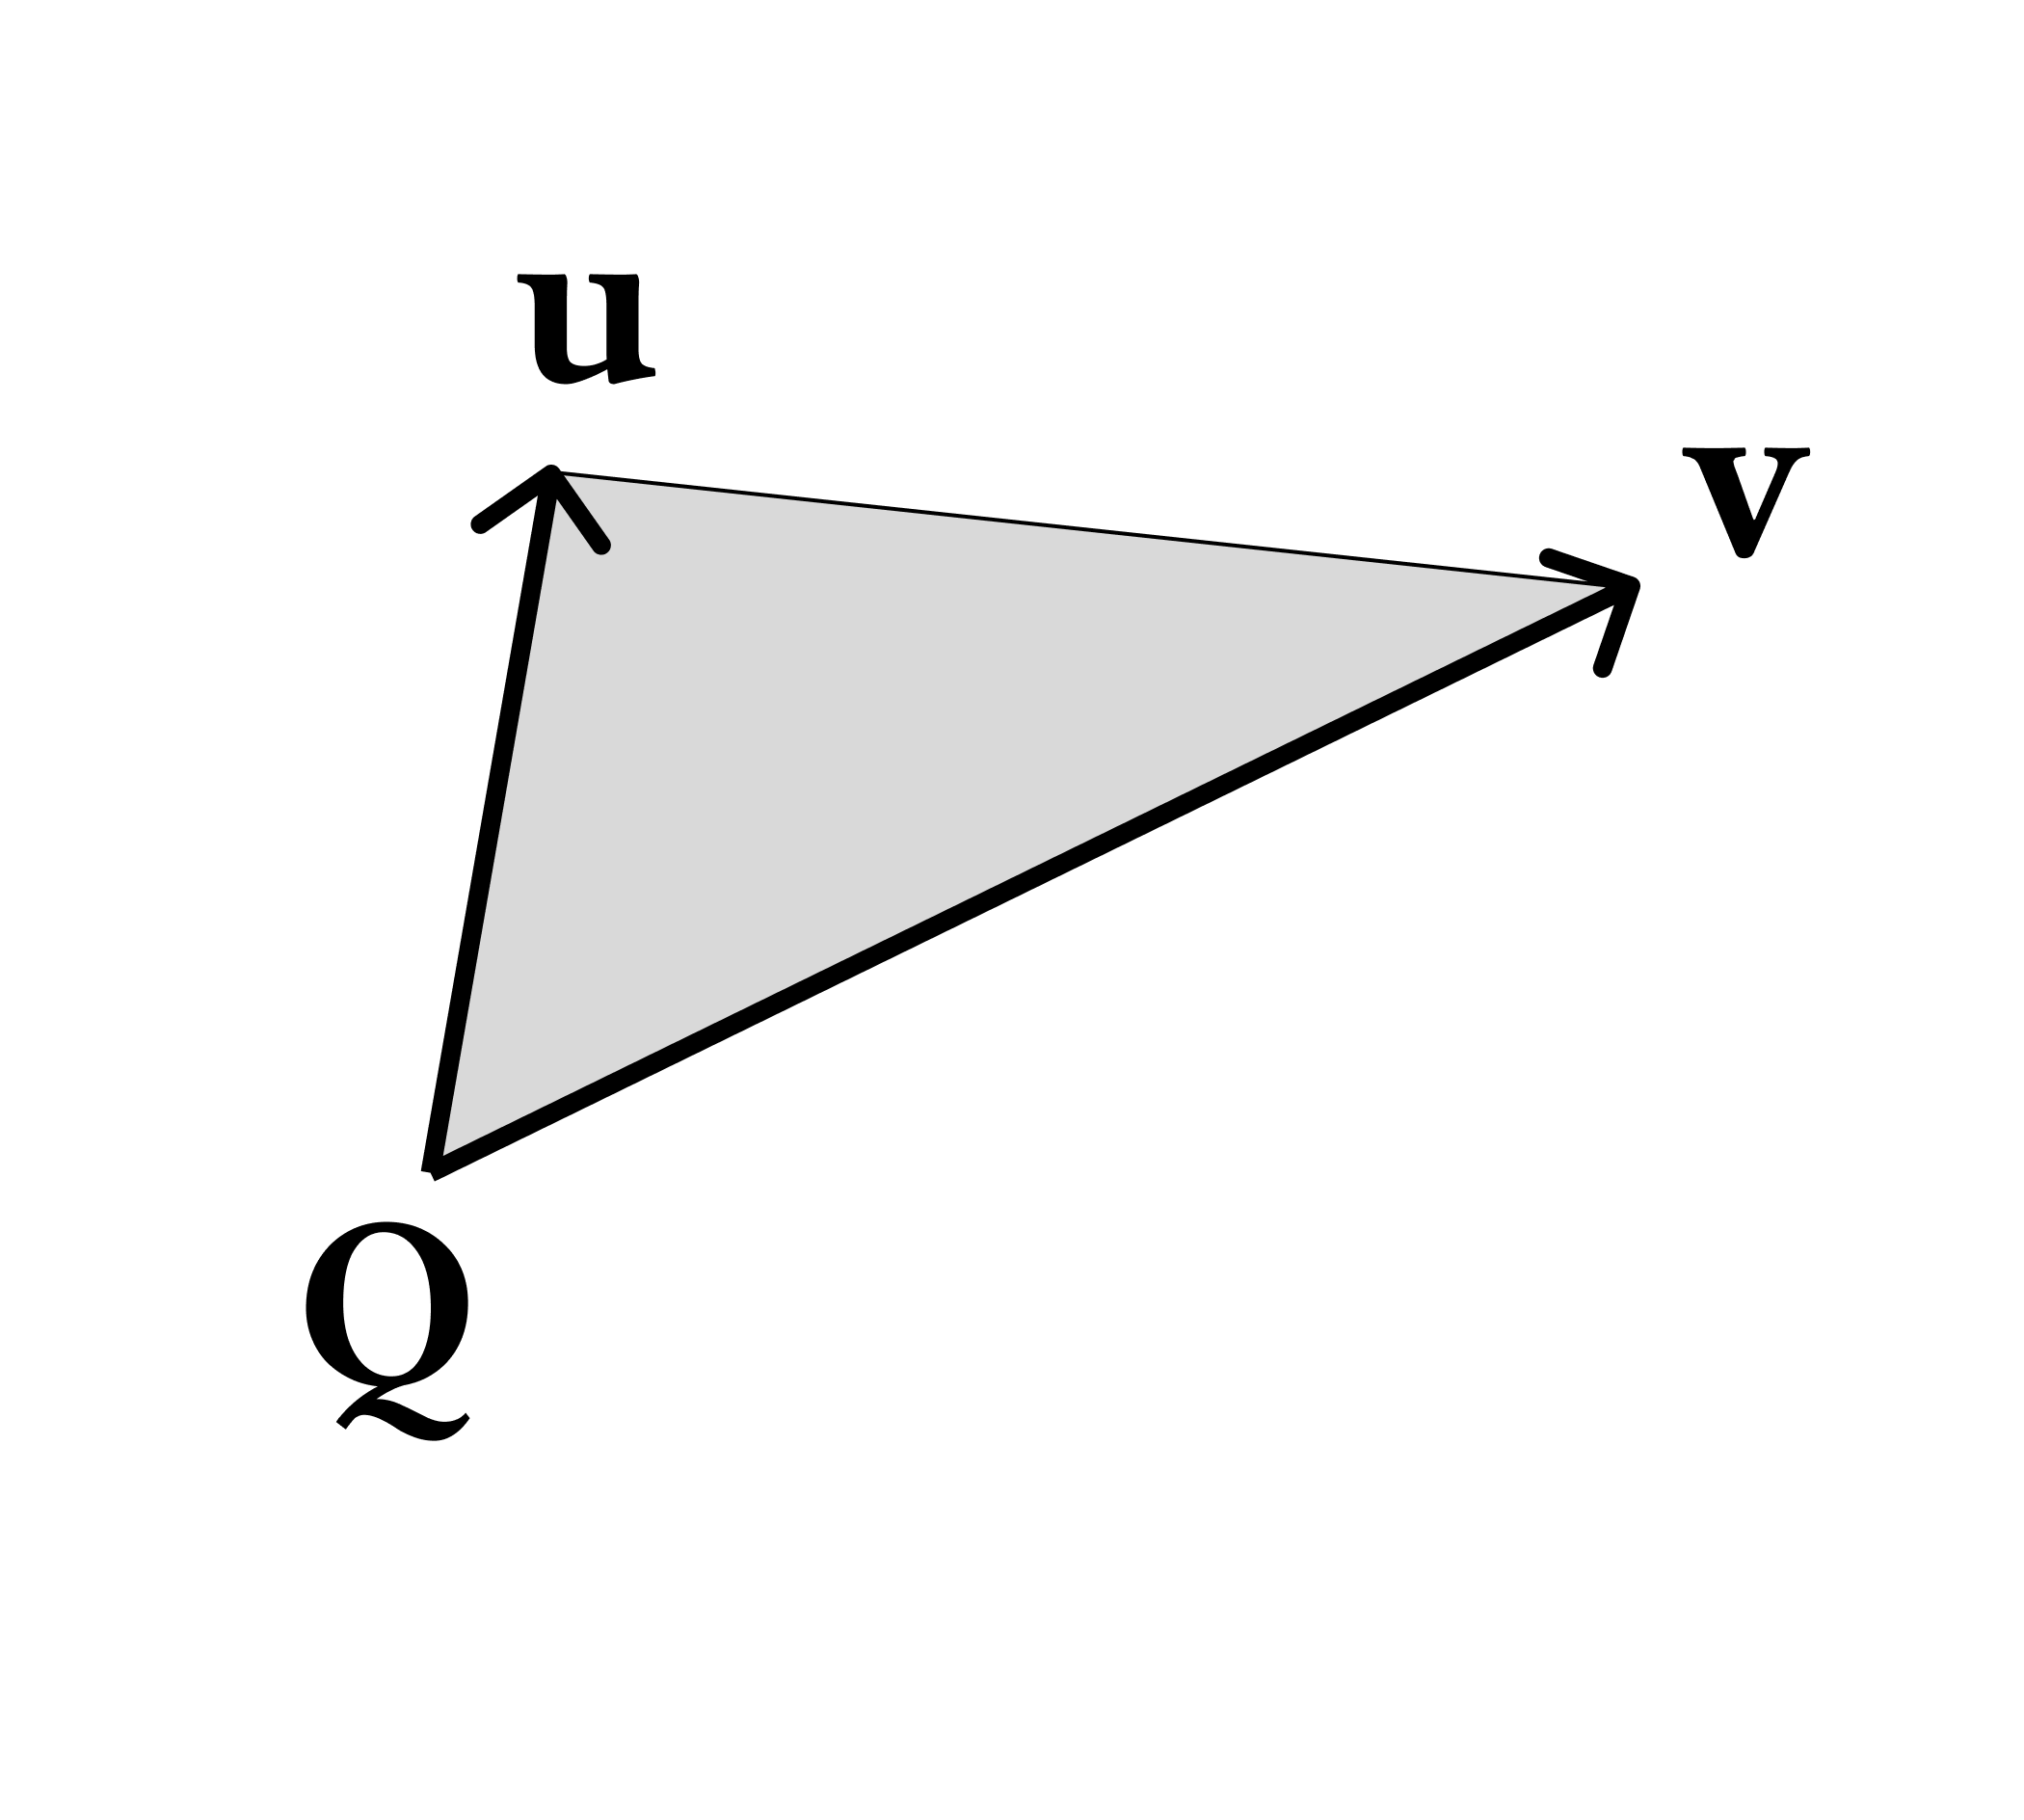
\includegraphics[width=0.25\textwidth]{resources/q-u-v-parameterization.png}
  \caption{Triangle defined using three vertices, $Q$ as the position and $u$,$v$ as direction vectors starting at $Q$.}
  \label{fig:q-u-v-parameterization}
\end{figure}

An alternative way to define a triangle is using three vertices, each in world space. The vertices can be defined as $v_1 = (x_1, y_1, z_1)$, $v_2 = (x_2, y_2, z_2)$ and $v_3 = (x_3, y_3, z_3)$. Converting between the two systems can be done using the following formulas:

\begin{equation}
  \label{eqn:triangle-vertices-to-q-u-v}
  Q = v_1
\end{equation}

\begin{equation}
  \label{eqn:triangle-vertices-to-q-u-v1}
  u = v_2 - v_1
\end{equation}

\begin{equation}
  \label{eqn:triangle-vertices-to-q-u-v2}
  v = v_3 - v_1
\end{equation}

\subsection{Frustum}

The frustum is a geometric shape which is used to define the camera's view. See \autoref{fig:camera-frustum} for a visual representation.

\begin{figure}[H]
  \centering
  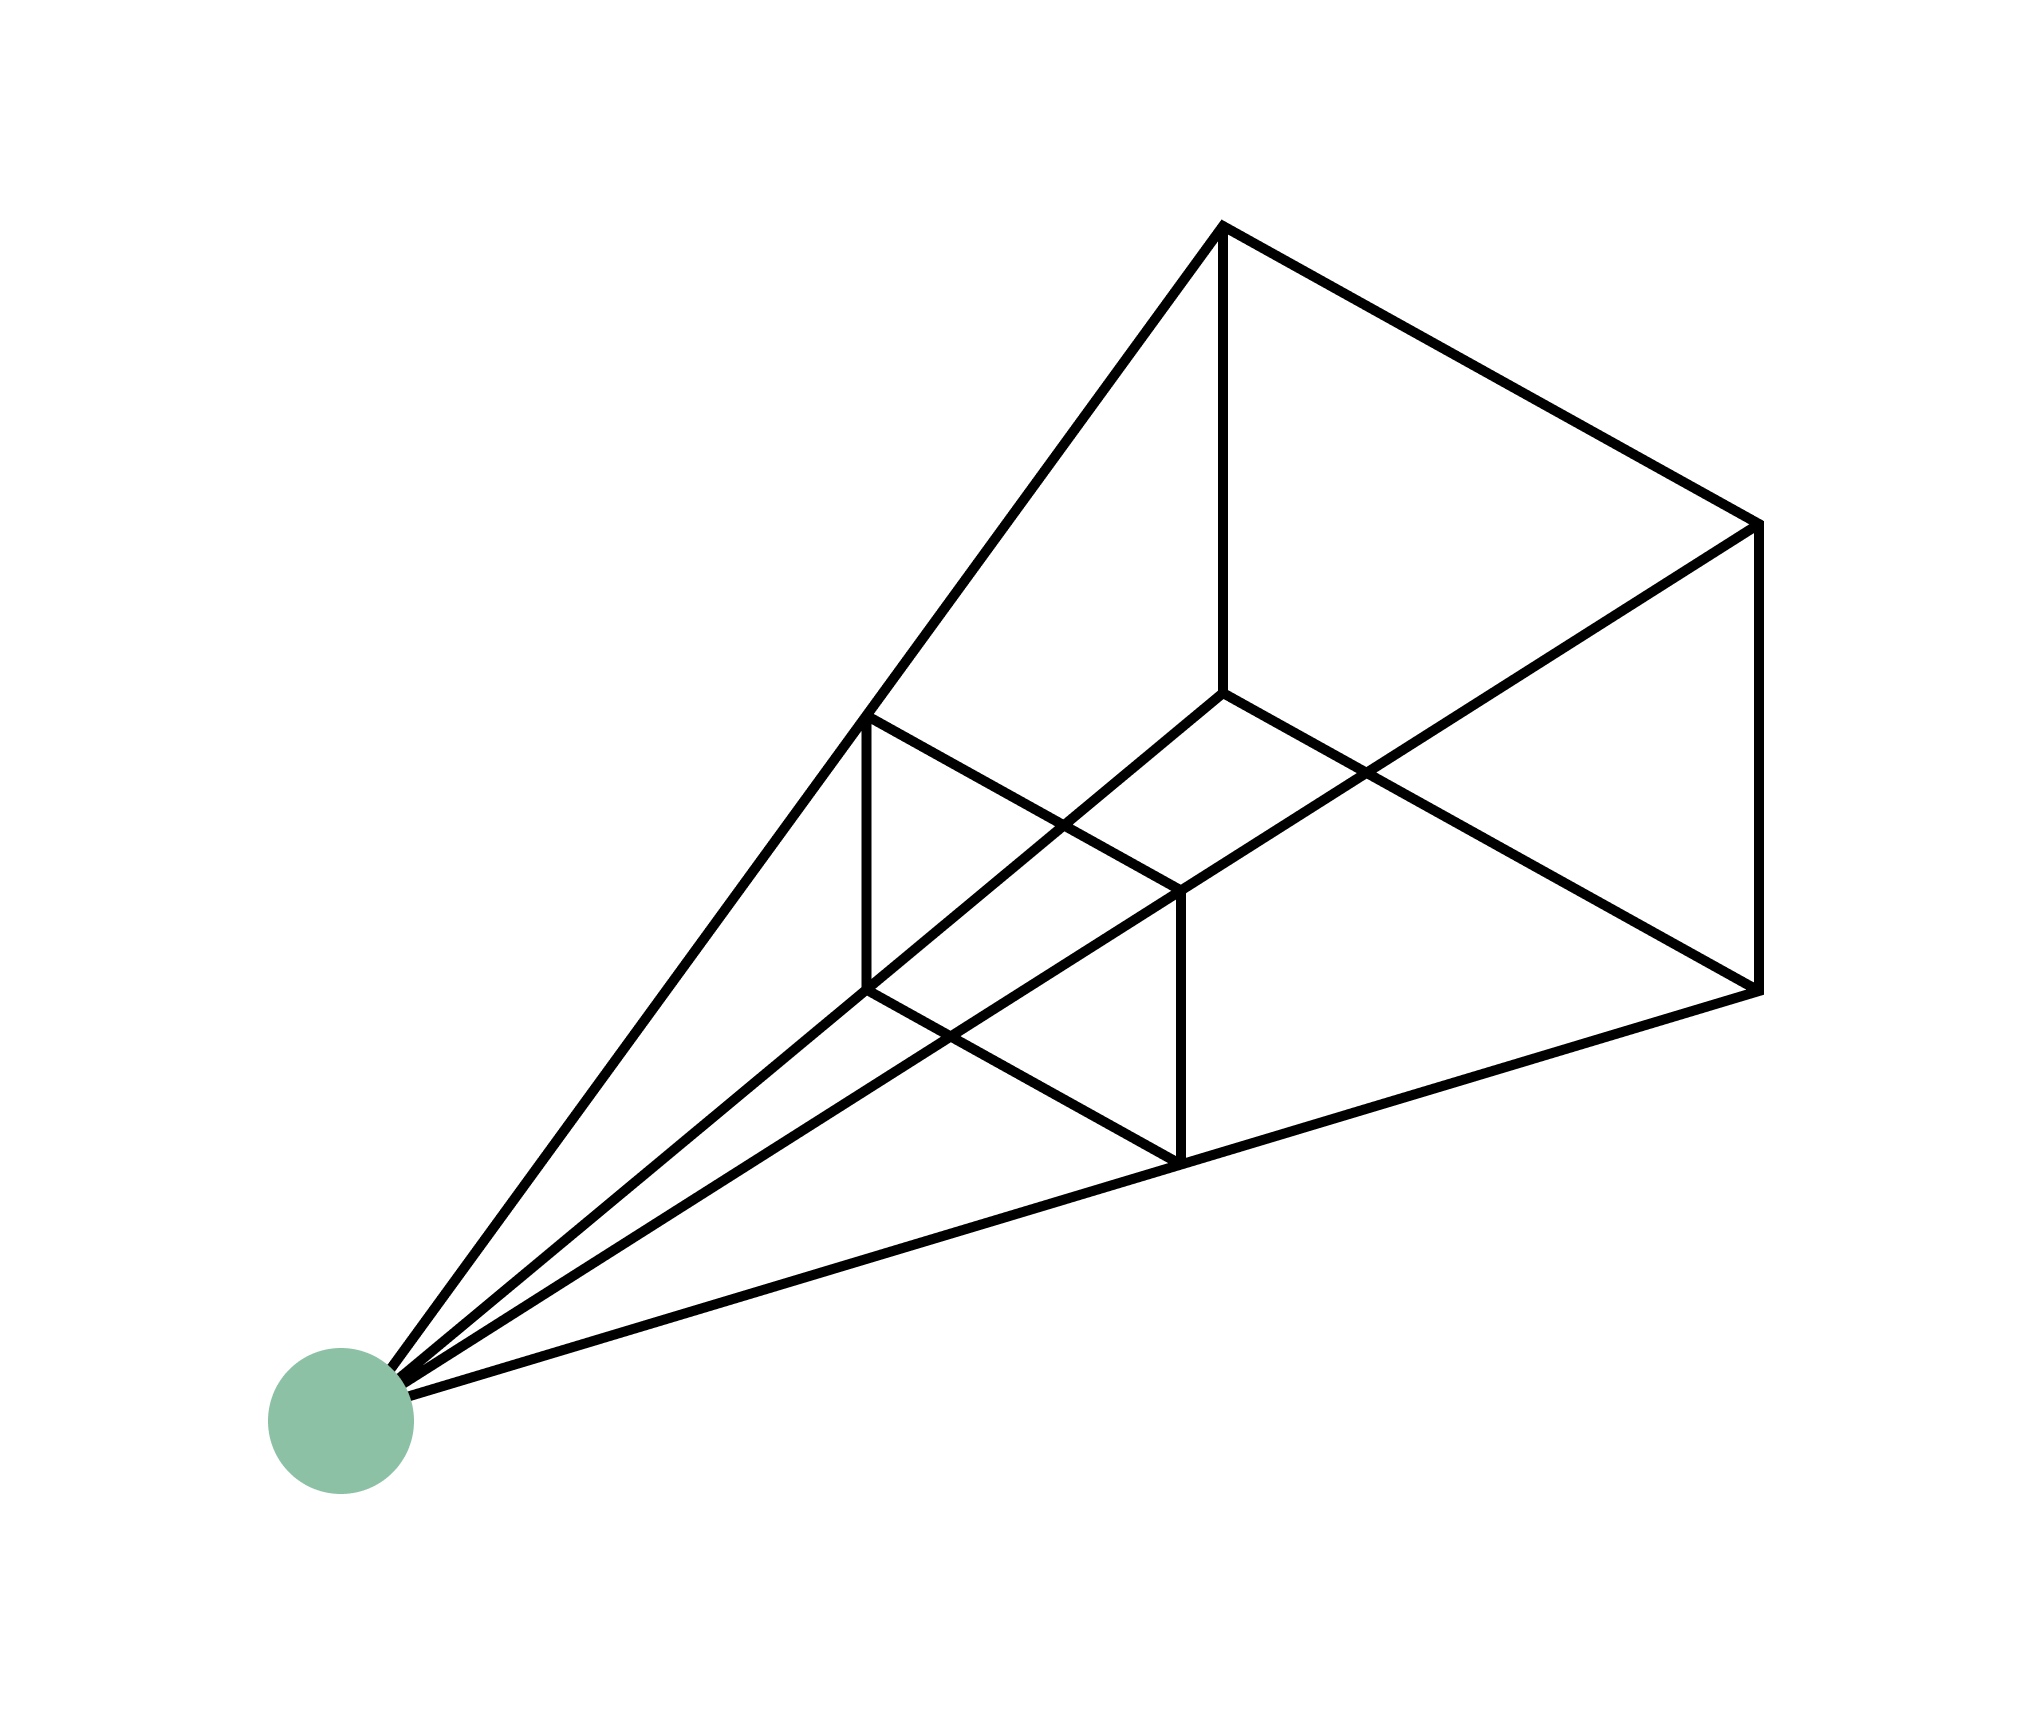
\includegraphics[width=0.25\textwidth]{resources/camera-frustum.png}
  \caption{Frustum shape, the green dot indicates the position of a camera in perspective projection.}
  \label{fig:camera-frustum}
\end{figure}

\section{Computer Graphics}

This section provides an overview of computer graphics, including its history, key concepts and applications.

Since the early days of computing, researchers have explored ways to process visual information using computers. While the field also encompasses aspects such as image processing or two-dimensional graphics, the main focus of this thesis is on three-dimensional computer graphics. While this includes topics such as animation, geometry processing, the main topics covered are geometry representation, rendering and shading.

\subsection{GPU}

The GPU is a specialized processor that is well-suited for workloads which require parallel processing. GPUs are widely used in computer graphics and other disciplines such as Machine Learning relying on parallel processing.

The first GPUs were developed in the 1990s and have since been integrated into most consumer hardware including smartphones, tablets, and laptops.

While CPU parallelization on consumer hardware is generally limited to a few cores, GPUs have thousands of compute units.

\subsection{Rendering Approaches}

In order to visualize 3d scenes using a computer, different rendering approaches have been developed. Two of the most common approaches are rasterization and ray tracing and will be described in more detail in the following sections.

\subsubsection{Rasterization}

Rasterization is a rendering technique which maps the geometry of a 3d scene onto a 2d plane. Historically, the technique has been widely adopted in real-time rendering due to its efficiency. However, there are inherent limitations in terms of realism.

One of the main limitations is the lack of support for global illumination. A related shortcoming is the difficulty to generate ambient occlusion. Certain techniques such as using pre-baked shadow, environment and light maps, screen space ambient occlusion (SSAO) \cite{bavoil2008ssao}, screen space directional occlusion (SSDO) \cite{ritschel2009ssdo} or ray traced ambient occlusion (RTAO) \cite{gautron2020rtao} have been developed to address these limitations.

To obtain reflections, one frequently used technique is multi-pass rendering. The idea is to first render the scene from the perspective of the reflective object and then render a second pass from the camera while leveraging the first pass as a texture.

These approaches induce complexity and can be computationally expensive. An alternative technique which resembles reality more closely could alleviate these issues: Ray Tracing.

\subsubsection{Ray Tracing}

Ray Tracing is a rendering technique which simulates light transport in a scene. The main idea is to cast rays from the camera into the scene and compute the color of the object the ray intersects with. By adding additional bounces of the light ray, the technique can simulate global illumination.

One of the earliest papers describing approaches to solve shadow casting was written as early 1968 by Appel \cite{appel1968shading}. The term global illumination was coined by Whitted in 1979 \cite{whitted2020OriginsOfGlobalIllumination}.

Due to the computational complexity of these algorithms, ray tracing was not widely adopted until the 1980s. Some of the first widely used ray tracing software was POV-Ray, which was released in 1991 \cite{POV_Ray_Documentation}. Blue Moon Rendering Tools (BMRT) \cite{bmrt}, a RenderMan compliant renderer, was released in the mid 90s and was one of the first ray tracing renderers to be used in the industry. In 2003 PRMan included ray tracing capabilities \cite{RenderMan_11_Release_Notes}.

The rendering equation has been defined in 1986 in a paper which also coined the term path tracing \cite{kajiya1986rendering}. Generally, path tracing can be seen as a Monte Carlo integration of the rendering equation which is defined as

\begin{equation}
  \label{eqn:rendering-equation}
  I(x, x') = g(x, x') [\epsilon(x, x') + \int_{S} p(x, x', x'')I(x', x'')dx'']
\end{equation}

Where $I(x, x')$ is the radiance from point $x$ to point $x'$. $x$ for example being the camera position and $x'$ the intersected object. $g(x, x')$ is a geometry term determining how much light is transmitted. This depends on the distance and possibly occlusions such as in the case of transparent surfaces. $\epsilon(x, x')$ is the emitted radiance, generally used for light sources. The integral term is taken over $S$ = $\cup S_i$ which is the union of all surfaces. $p(x, x', x'')$ is the bidirectional reflection function which describes how light is reflected at the surface. \cite{kajiya1986rendering}

Further research into light transport techniques such as bidirectional ligh transport or Metropolis Light Transport has been conducted in the 1990s \cite{veachMonteCarloLightTransport}.

\todo{This is only for showing citation style}

\subsubsection{Aliasing}

Aliasing is a common issue in computer graphics. It occurs when the resolution of the screen is not sufficient to represent the scene accurately. One such example is jagged edges on diagonal lines. Anti-aliasing techniques can be employed to reduce the effect.

In ray tracing, aliasing can be alleviated by randomizing the direction of the rays.

\subsection{Graphic APIs}
\subsubsection{OpenGL}

OpenGL is an API for rendering 3d graphics. After its introduction in 1992, it was widely adopted. Subsequently, the standard has been ported to other platforms and has been extended with new features.

To date, OpenGL is still widely used in the industry, but it has been replaced by more modern APIs in recent years.

\subsubsection{Vulkan, Metal, DirectX}

While OpenGL and derivatives such as OpenGL ES have been widely adopted, the introduction of a number of new APIs has changed the landscape. Some of the most notable APIs are:

\begin{itemize}
    \item{Vulkan} Developed by the Khronos Group, Vulkan is a low-level API which is supported on a wide range of platforms.
    \item{Metal} Developed by Apple, Metal is a low-level API which is supported on Apple platforms.
    \item{DirectX} Developed by Microsoft, DirectX is a collection of APIs which are supported on Windows platforms.
\end{itemize}

\subsubsection{WebGL}

WebGL is a graphics API based on OpenGL ES 2.0 for the web. It was initially released in 2011 and has since been adopted by all major browsers.

WebGL is designed to offer a rendering pipeline, but does not offer GPGPU capabilities. There have been efforts to extend with compute shaders, but efforts by the Khronos Group have been halted in favor of focusing on WebGPU instead.

In order to provide GPGPU capabilities, workarounds have been developed. The basic idea is to render the output of a fragment shader to a texture and interpreting the output as binary data instead of color information.
There are libraries such as GPU.js which provide GPGPU capabilities using WebGL. Tensorflow.js, a library for training and deploying Machine Learning models, use similar techniques in the WebGL backend.

Since its introduction, WebGL has been extended with new features. WebGL 2.0, which is based on OpenGL ES 3.0, was released in 2017. Of the major browsers, Safari was the last to support it out of the box in 2021. Since WebGL 2.0 no new major versions have been released but new features have been added.

\section{WebGPU}

WebGPU is a new web standard which is no longer based on OpenGL. One of the main capabilities is support for GPGPU by design. While all major browser vendors have announced intent to support WebGPU, to date only Chrome has shipped WebGPU for general use on desktop as well as mobile.
The standard is still in development and new features are being added.
Common 3d engines such as Babylon.js, Three.js, PlayCanvas and Unity have announced support for WebGPU.

\subsection{Buffers}

Data needs to be transferred between the CPU and the GPU. Buffers are the primary method to do so. Depending on the type of data to be transferred, different types of buffers can be used.

\subsubsection{Uniforms}

Uniform Buffers are optimized for data which is read-only on the GPU and is the same for all vertices or fragments. Such information could be the projection matrix.

\subsubsection{Storage}

Storage Buffers are intended for read-write access on the GPU. The limits of the buffer are higher than for uniform buffers.

\subsubsection{Vertex}

\subsubsection{Index}

\subsection{Shading Language}

WebGPU introduces a new shading language called WebGPU Shading Language (WGSL). The language is statically typed and supports a variety of data structures required for computer graphics as well as general-purpose computing.

WGSL supports common high-level helpers such as Swizzling, which is a class of operations which facilitate managing vector elements. For example, given a vector \verb|let v = vec3f(x, y, z)|, the operation \verb|v.xy| returns a vector \verb|(x, y)|.

\subsubsection{Memory Alignment}

WGSL supports \verb|struct| for defining data structures. However, when passing data between the CPU and the GPU, memory alignment needs to be considered. Alignment is a constraint, restricting the memory address at which a data structure can be stored. Having strict memory alignment enables use of more efficient hardware instruction sets, or address hardware requirements.

Each type in WGSL has specific alignment requirements which are independent of the size. For example, a \verb|vec3f| has a size of 12 bytes, but requires an alignment of 16 bytes. So for a struct definition such as can be seen in \autoref{code:memoryAlignment}, the struct requires 32 bytes of memory to store 20 bytes of data as illustrated in \autoref{fig:memory-alignment}. The excess 12 bytes are used for padding.

\begin{figure}[H]
  \begin{lstlisting}[style=wgsl]
  struct ThreeFields {
    a: f32,
    b: vec3f,
    c: f32
  }
  \end{lstlisting}
  \caption{WGSL \texttt{struct} containing three fields of type \texttt{f32} and \texttt{vec3f}.}
  \label{code:memoryAlignment}
  \end{figure}

\begin{figure}[H]
  \centering
  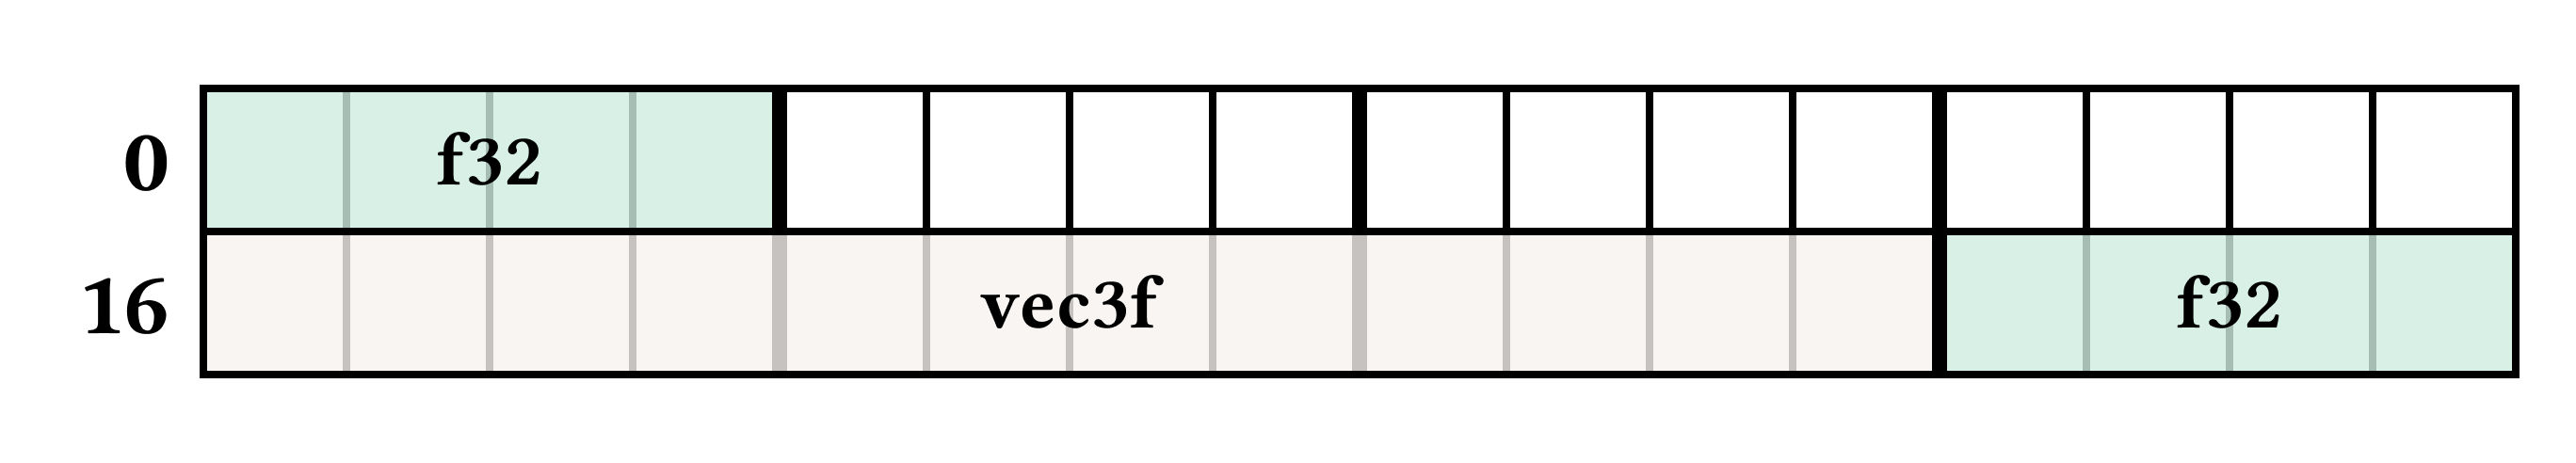
\includegraphics[width=0.8\textwidth]{resources/memory-alignment.png}
  \caption{Memory Alignment with padding for struct defined in \autoref{code:memoryAlignment}.}
  \label{fig:memory-alignment}
\end{figure}

Memory alignment is opaque while writing WGSL code, it is relevant when providing data to the GPU. For creating buffers, the alignment requirements need to be considered. When using JavaScript to create buffers, the standard Web APIs such as \texttt{Float32Array} or \texttt{Uint32Array} can be used to provide data. In order to write data to the \texttt{struct} in \autoref{code:memoryAlignment}, the views can be created as shown in \autoref{code:memoryAlignmentJs}.

\begin{figure}[H]
  \begin{lstlisting}[style=JavaScript]
const ValueBuffer = new ArrayBuffer(32);
const a = new Float32Array(ValueBuffer, 0, 1);
const b = new Float32Array(ValueBuffer, 16, 3);
const c = new Float32Array(ValueBuffer, 28, 1);
  \end{lstlisting}
  \caption{JS code providing views to access the \texttt{struct}.}
  \label{code:memoryAlignmentJs}
\end{figure}

\section{Optics}

In physics, optics is the study of light. The field encompasses topics such as light propagation and optical properties of matter. \cite{fowles1989introduction}

\section{Ray Tracing}
\subsection{Monte Carlo Ray Tracing}
\subsection{Intersection Testing}

When casting a ray into the scene, the first step in a ray tracer is to determine where the ray intersects with the geometry of the scene.

A brute force approach could be to determine the intersection distance for each object to the ray and picking the one with the lowest distance. Given the fact, that common objects consist of thousands of triangles and ray tracing many rays, this approach is not efficient.

In order to accelerate the intersection testing, various approaches have been developed.

The \fgls{BVH}{\e{Bounding Volume Hierarchy}, common tree-based acceleration structure} is an acceleration structure which is leveraged to speed up the ray intersection tests. The core idea is to group adjacent objects in a bounding volume and structure the hierarchy in a way that all child elements of a node are contained in the bounding volume of the parent node. This allows for early rejection of branches which are not intersected by the ray. By employing a BVH, the number of intersection tests can be reduced from $O(n)$ to $O(log(n))$.

\subsection{Importance Sampling}

\section{Physically Based Rendering}

Defining the geometry is one part of the equation. Another major part is defining materials. Materials define how a surface interacts with light. The core idea of physically based rendering (PBR) is to simulate the interaction of light using physical models. Instead of fine-tuning parameters for a specific look and feel and having to adjust based on desired lighting situations, PBR aims to define a material which behaves consistently in different lighting situations.

\subsection{BxDF}
\subsection{Microfacet Theory}

While the macroscopic appearance of a material is visible to the human eye, the microscopic structure of the material is crucial in determining how light interacts with the material. Microfacet theory is a model which describes this microscopic structure. The distribution of the normals of the microfacet is described by a distribution function.

\section{Exchange Formats}

In order to exchange 3d scenes between a multitude of applications, various standardized formats have been developed. These formats are optimized for different use cases depending on the requirements of the application.

\subsection{General Purpose Formats}

One of the most widely used formats is Wavefront OBJ which was established in the 1980s. The format is text-based and has basic support for materials and textures. However, it lacks support for more advanced features such animations. Additionally, due to its encoding, it is not well-suited for delivery over the web compared to more modern alternatives.

Formats such as the proprietary FBX by Autodesk established in 2006 can address the shortcomings in terms of advanced features. The format is supported by a wide range of applications.

\subsection{Interoperability Formats}

Other formats such as COLLADA have been developed to improve transporting 3d scenes between different applications. It is XML-based and has been established in 2004.

Since, other formats such as USD and has been open-sourced by Pixar in 2016.

\subsection{Runtime Formats}

For usage in end-user applications, such as for this thesis, the glTF format is well-suited. It has been established in 2015 and is designed to be efficient for transmission and loading of 3d scenes.

\section{Material Description}

A variety of standardized material description models have been developed over the years.

\subsection{MaterialX}

MaterialX is an open standard which was originally developed by Lucasfilm in 2012. The standard has since been adopted by the Academy Software Foundation as an open standard.

While not strictly limited to PBR, the standard provides a wide range of features to describe physically based materials \cite{Harrysson2019}.

\subsection{OpenPBR}

OpenPBR is hosted by the Academy Software Foundation as an open standard. It differs from MaterialX in that it is providing an über-shader approach instead of a node-based approach. It serves as a combination of Autodesk Standard Surface and Adobe Standard Material and is being worked on by both companies. The über-shader approach is defined by having a fix set of inputs which can be adjusted, but it does not allow for custom node graphs as MaterialX does.
